\documentclass[11pt, a4paper]{article}\usepackage[]{graphicx}\usepackage[]{color}
%% maxwidth is the original width if it is less than linewidth
%% otherwise use linewidth (to make sure the graphics do not exceed the margin)
\makeatletter
\def\maxwidth{ %
  \ifdim\Gin@nat@width>\linewidth
    \linewidth
  \else
    \Gin@nat@width
  \fi
}
\makeatother

\definecolor{fgcolor}{rgb}{0.345, 0.345, 0.345}
\newcommand{\hlnum}[1]{\textcolor[rgb]{0.686,0.059,0.569}{#1}}%
\newcommand{\hlstr}[1]{\textcolor[rgb]{0.192,0.494,0.8}{#1}}%
\newcommand{\hlcom}[1]{\textcolor[rgb]{0.678,0.584,0.686}{\textit{#1}}}%
\newcommand{\hlopt}[1]{\textcolor[rgb]{0,0,0}{#1}}%
\newcommand{\hlstd}[1]{\textcolor[rgb]{0.345,0.345,0.345}{#1}}%
\newcommand{\hlkwa}[1]{\textcolor[rgb]{0.161,0.373,0.58}{\textbf{#1}}}%
\newcommand{\hlkwb}[1]{\textcolor[rgb]{0.69,0.353,0.396}{#1}}%
\newcommand{\hlkwc}[1]{\textcolor[rgb]{0.333,0.667,0.333}{#1}}%
\newcommand{\hlkwd}[1]{\textcolor[rgb]{0.737,0.353,0.396}{\textbf{#1}}}%
\let\hlipl\hlkwb

\usepackage{framed}
\makeatletter
\newenvironment{kframe}{%
 \def\at@end@of@kframe{}%
 \ifinner\ifhmode%
  \def\at@end@of@kframe{\end{minipage}}%
  \begin{minipage}{\columnwidth}%
 \fi\fi%
 \def\FrameCommand##1{\hskip\@totalleftmargin \hskip-\fboxsep
 \colorbox{shadecolor}{##1}\hskip-\fboxsep
     % There is no \\@totalrightmargin, so:
     \hskip-\linewidth \hskip-\@totalleftmargin \hskip\columnwidth}%
 \MakeFramed {\advance\hsize-\width
   \@totalleftmargin\z@ \linewidth\hsize
   \@setminipage}}%
 {\par\unskip\endMakeFramed%
 \at@end@of@kframe}
\makeatother

\definecolor{shadecolor}{rgb}{.97, .97, .97}
\definecolor{messagecolor}{rgb}{0, 0, 0}
\definecolor{warningcolor}{rgb}{1, 0, 1}
\definecolor{errorcolor}{rgb}{1, 0, 0}
\newenvironment{knitrout}{}{} % an empty environment to be redefined in TeX

\usepackage{alltt}
\usepackage{graphicx}
\usepackage{lipsum}
\usepackage{verbatim}
\usepackage[vmargin=3cm, hmargin=2cm]{geometry}
\usepackage{url}
\usepackage{hyperref}
\usepackage{fancyhdr}
\usepackage{color}
\usepackage{amsmath, amssymb}
\usepackage{longtable}
\usepackage{lscape}
\usepackage{natbib}
\usepackage{xspace}
\usepackage{textcomp}
\usepackage{float}
\usepackage{booktabs}
\usepackage{subcaption}
% =======================================

% bibliography
\bibliographystyle{apalike}
\IfFileExists{upquote.sty}{\usepackage{upquote}}{}
\begin{document}
\tableofcontents
\newpage
\section{Introduction}
Cells are one of the fundamental units of life. They show an immense complexity and diversity. Their identity and function is determined by environmental stimuli, the physical environment, the cell cycle and neighbouring cells \citep{wagner2016revealing}. Only recently has it been possible to investigate the transcriptome of a single cell. Single-cell RNA sequencing (scRNA-seq) was first published by \citet{tang2009mrna}. This method addresses new biological issues, such as the identification of rare cell populations, and allows us to measure the frequency of cell types in tissues, characterise differences in similar cell types and investigate the heterogeneity of cell states or cell lineages \citep{andrews2017identifying}.

A typical scRNA-seq workflow consists of the isolation of single cells, the extraction of RNA, cDNA library preparation, and the amplification and sequencing of the libraries. A wide variety of scRNA-seq protocols exists, differing in throughput, full transcript or 3' sequencing, costs and automatisation. Small-scale protocols are standard PCR plate-based methods or methods in which cell isolation and library preparation are combined into one protocol. A typical small-scale method is the PCR plate-based SMART-seq2 \citep{picelli2013smart}. Libraries are full-transcript sequenced using a standard Illumina sequencing approach. Typically, hundreds of cells are processed and ERCC is used for normalisation. On the other side of the spectrum are droplet-based methods such as Drop-seq and 10xChromium, which allow the processing of thousands of cells.

The differences between scRNA-seq and bulk experiments are the lower sequencing depth (100,000--5 million reads per cell), higher variability and more outliers. scRNA-seq data suffers from technical noise, batch effects and low capture efficiency. Batch effects occur when different biological conditions are processed in different batches, making the deconvolution of technical noise and biological effect impossible. This should be avoided by an appropriate experimental design that allows for the statistical deconvolution between unwanted and wanted variation. In scRNA-seq the single experimental unit is the cell, making it not always possible to use this approach. Different cells in an experiment may need different sample processing, or their biological differences may affect the downstream analyses.

The starting amounts of the library preparation can be as low as ten picogrammes of total RNA \citep{picelli2013smart}. Two main issues are arising due to the low starting amount are  overamplification and low capture efficiency. Low and moderate expressed genes are not captured during the reverse transcription, which leads to dropouts of genes and a zero-inflated gene expression. scRNA-seq data has an excess of zero counts, which can be split into systematic, semi-systematic and stochastic zeros \citep{lun2016pooling}. Systematic zeros and semi-systematic zeros come from genes that are silent in a subpopulation or across all cells, respectively. 
Stochastic zeros are zero counts that have been obtained due to sampling. They affect genes with a count distribution near zero and have to be dealt with the normalisation steps.  
 
To deal with technical noise Unique Molecular Identifiers (UMI) or spike-in from the External RNA Control Consortium  (ERCC) are used. UMI are short random barcodes attached to the single-stranded cDNA in the reverse transcriptase process. By counting the unique UMI reads aligned to the genome an estimated tag count is obtained. Spike-in are added before amplification. Under the assumption that the amplification of the endogenous and exogenous RNA is similar, they can be used for library size normalisation and to remove technical noise. 

In general, scRNA-seq experiments consist of high-dimensional data. High-dimensional data suffers from the curse of dimensionality \citep{wagner2016revealing}. Distances in high-dimensional data become unstable and subpopulations cannot be separated \citep{andrews2017identifying}. Additionally, computational requirements are high. Reduction of the dimension is made by two approaches. Using linear or non-linear projections of the data from the original high-dimensional to a lower-dimensional space, or by feature selection, in which uninformative genes are removed.

The detection of new cell types is one of the most common aims for scRNA-seq data. Lately, a broad spectrum of clustering methods have been specifically developed for the clustering of single cells.
The aim of this study is to evaluate clustering methods for scRNA-seq data. 
\section{Methods}

\subsection{Dimension reduction}
All methods require a dimension reduction step before clustering. Commonly used methods are either Principal Component Analysis (PCA) or t-distributed Stochastic Neighbour Embedding (tSNE). PCA finds a rotation of the original data in which the newly obtained first coordinates have the highest possible variance, the second coordinates the second-greatest variance etc. Practically, PCA is computed by spectral decomposition of the correlation matrix. Dimension reduction is achieved either by selecting only the first few PCs whose eigenvalues are less than average, or by determineing the number graphically by plotting the eigenvalues. PCA is deterministic and relatively fast but restricted to linear spaces.

In contrast,  tSNE is a non-linear mapping \citep{van2013barnes}. Stochastic neighbour embedding (SNE) transforms Euclidean distances to conditional probabilities $p_{j|i}$. That is the probability of \(x_j\) is the nearest neighbour of $x_i$ under a Gaussian centred at $x_i$. The low-dimensional counterpart $q_{i|j}$ is similar with a Gaussian centered at $y_i$ and variance of $1/\sqrt(2)$. SNE minimises the divergence between $p_{j|i}$ and $q_{j|i}$ using the Kullback-Leiber divergence. tSNE implements a Student's t-distribution for the low dimensional space and a symmetric version of the cost function to simplify optimisation and to overcome the crowding problem. In tSNE, the cost function uses the joint probabilities $p_{ij}$ and $q_{ij}$ instead of conditional probabilities. To deal with large datasets, the Barnes-Hut implementation uses random walks on the nearest neighbour network with a PCA step to reduce the dimensionality of the high-dimensional data. tSNE is stochastic, depends on a perplexity parameter and distances between clusters are not preserved. 
\subsection{Clustering methods}
Identifying unknown cell populations is one of the main uses of scRNA-seq data \citep{andrews2017identifying}. Eleven clustering methods have been evaluated for this study. These methods and algorithms can be roughly classified into three groups: K-means, graphclustering and hierarchical-based clustering. 
SC3, SIMLR, Linnorm and RaceID use k-means in different fashions, while pcaReduce and CIDR are based on hierarchical clustering. The graph-based methods are SNN-Cliq and Seurat. An overview of the methods is given in Table \dots
\paragraph{K-means}
K-means clustering finds a predefined number of centres $k$ and cell assignments, such that their within-group sum of squares is minimised \citep{hartigan1979algorithm}. $k$ cluster centres are randomly assigned.
Each data point is then assigned to the nearest centre using Euclidean distances. The centres are then recomputed using the average of the data points that are assigned to each of the $k$ centres. This procedure is iterated until the algorithm converges. The assigning of the centres is random. Also, it's not guaranteed to find the global minimum.  The drawbacks of the method are that it assumes spherical cluster and the sensitivity to scaling. 
\paragraph{pcaReduce}
pcaReduce uses k-means clustering to find the number of clusters in the reduced dimension given by PCA \citep{yau2016pcareduce}. The main assumption is that large classes of cells are contained in low-dimension PC representation and more refined subsets of these cells types are contained in higher-dimensional PC representations. Given a gene expression matrix, the clustering algorithm starts with a k-means clustering on the PCA projections $Y_{n\times q}$ with $q+1$ clusters. Where $n$ are the cells and $q$ are the number of PCs. The number of initial clusters $k$ is typically around 30,  guaranteeing that most cell types are captured. For all pairs of clusters, the joint probabilities are computed. Two clusters are merged by selecting the pair with the highest joint probability or by sampling proportionally by the joint probabilities. The number of clusters is now decreased to $K-1$. Next, the PC with the lowest variance is deleted and a k-means clustering with $K-2$ centres is performed. This process is repeated until only one single cluster remains. When using pcaReduce $q$ cluster partitions with $k-1$ clusters are obtained.
\paragraph{SC3}
Implemented in the SC3 method is a gene- and cell-filtering, as well as a log transformation step of the expression matrix \citep{kiselev2017sc3}. The filtered expression matrix is then used to compute  Euclidean, Pearson and  Spearman dissimilarity measures. By PCA or Laplacian graphs a lower-dimensional representation of the data is obtained.  K-means clustering is then performed on the different dimensions. Next, a consensus matrix of the different clustering results is computed. The consensus matrix is a binary similarity matrix with entry one if two cells belong to the same cluster and zero otherwise. The consensus matrix is obtained by averaging the individual clustering. The last step is a hierarchical clustering step with complete linkage. The cluster is inferred by the $k$ level of hierarchy, where $k$ is supplied by the user. To reduce runtime SC3 changes the clustering method when supplied with more than 5'000 cells. Randomly selected cells are then used for the clustering approach described above. These subpopulations are then used to train a support vector machine to infer the remaining cells.
\paragraph{SNNcliq}
SNNcliq computes a shared nearest-neighbour-graph based on the high-dimensional data \citep{xu2015identification}. The nodes are the data points and the weighted edges are the similarities between the data points. Cells are defined as a cluster if they have a defined number of edges between them, forming a "clique". 

A similarity matrix using Euclidean or other similarity measures is then computed. Using this similarity matrix, the k-nearest-neighbours (KNN) for each data point are listed. The number of nearest neighbours has to be supplied by the user. Edges between data points are assigned if they share at least one KNN. The weights of the edges are defined by a function of the number of nearest neighbours and their respective ranks. 
Identification of clusters is made by finding quasi-cliques associated with each node and merging them to unique clusters by the use of a greedy algorithm. A node induces a subgraph, which consists of all neighbour nodes and edges. For each node, a local degree is computed and a node is removed from the subgraph if its degree is lower thana given threshold which is proportional to the size of the clique. The threshold is supplied by the user and is typically set to 0.7. Next, the degrees between the nodes are recomputed and the process is repeated until no more nodes can be removed. A subgraph is assigned to a quasi-clique if it contains more than three nodes. To reduce redundancy, quasi-cliques that are completely included in other cliques are removed as well.
Clusters are then identified by merging the quasi-cliques. For each pair, an overlapping rate is computed. If it exceeds a predefined threshold $m$ the sub graphs are merged. Merging in different orders leads to different results, so pairs with larger sizes are prioritized.
\paragraph{SIMLR}
Most clustering methods rely on standard similarity metrics like Euclidean distances \citep{wang2017visualization}. SIMLR uses a weighted function of multiple kernels to compute a distance matrix. The assumptions is that the matrix has a block-diagonal structure, where the blocks represent the clusters $c$. The kernels are Gaussian kernels with a range of hyperparameters defining the variance of each kernel. The similarities are then used for data visualisation with tSNE or clustering using k-means on the latent space representations of the similarities.

\paragraph{CIDR}
Clustering through Imputation and Dimensionality Reduction (CIDR) takes the high dropout rate in scRNA-seq data into account \citep{lin2017cidr}. The method splits the squared Euclidean distance into three terms. These consist of one term in which both genes $k$ for the cell pairs $i$ an $j$ are non-zero, a second term in which one gene is zero and a third where both are zero. The authors state that only the cases where one gene is zero have a strong influence on the distances and the subsequent dimension reduction and clustering. To reduce the dropout-induced zero inflation, the method imputes the third term by its expected value given the distribution of the dropouts. 
The algorithm works basically in five steps: (i) Find features that are dropout candidates. That is genes that show an expression level below a threshold $T$. (ii) Find the empirical dropout probability $\hat P(u)$ using the whole data set. (iii) Calculate the dissimilarity using Euclidean distances together with pairwise a imputation process. Features that fall below the threshold $T$ are imputed using a weighting function. The weighting is based on the probability of being a dropout. (iv) Perform dimension reduction using PCA on the imputed distance matrix. (v) Perform hierarchical clustering using the first few PCs. The number of PCs can be determined by several methods. Here, we use an implemented variation of the scree method. 
\paragraph{Seurat}
Seurat uses raw counts, where filtering is both done gene- and cell-wise. A user-specified threshold for the minimum number of expressed features per cell and the minimum number of gene-wise expression per cell. Scaling, log transformation and normalisation of the counts is done with a scale factor of $10000$, a log2 transformation.... In the second gene-filtering step, low-variance genes are filtered out. 
Clustering is done using a PCA-latent space representation, which is used to compute the Jaccard distances. The Louvain algorithm then is used for clustering.

and a smart local moving algorithm (SLM). Here a resolution parameter defines the number of clusters.
\paragraph{Linnorm }
Linnorm is a normalisation and transformation method for count data \citep{yip2017linnorm}. The main assumption is that a homogeneously expressed gene-set exists. Using this gene subset, and by ignoring zero counts, the normalisation and transformation parameters are calculated. After normalisation, the expression values should show both homoscedasticity and normality. Linnorm includes functions for subpopulation analysis by t-SNE or PCA dimension reduction and subsequent k-means or hierarchical clustering. 

First, the values are scaled according to library size. Low count genes and genes that show high technical noise are filtered out. By default, genes showing a non-zero expression in at least 75 \% of the cells are retained. Note that this threshold is set to maintain at least three non-zero cells per gene, in order to calculate the skewness of the gene distributions. By gradually increasing this threshold only genes which show a negative correlation between the mean and the standard deviation (SD) is assured. 
A locally weighted scatterplot smoothing (LOWESS) curve is fitted on the mean versus SD relationship. The SD is scaled and outliers based on the SD are removed. Next, genes that show a high skewness are filtered out. The data is then transformed using a modified log transformation.
\paragraph{TSCAN}
TSCAN uses a pseudo-time algorithm for cell ordering \citep{ji2015tscan}. PCA dimension reduction on the preprocessed gene expression data is performed. Preprocessing is done by log transformation and by adding a pseudo-count. Low expressed genes are filtered out based on the zero-proportion and their covariance. Clustering is done by model-based clustering. 
The travelling salesman problem (TSP) is then solved by a minimum spanning tree. The user can then define the start/end point through the available biological information and compute a pseudo-time ordering score. 
\paragraph{ZINB-WaVE}
The method models the counts as an a zero-inflated negative binomial (ZINB) model that accounts for the zero-inflated, over-dispersed nature of scRNAseq count data\citep{risso2017zinb}. The model allows for the adjustment of gene- and cell-level confounders. 
Based on the preprocessing steps genes with less than five counts per feature are filtered out. Additionally, it is recommended to use only high variable genes.
\newpage
\subsection{Datasets}
The datasets Kumar, Trapnell and Koh were downloaded from the \textit{conquer} repository \url{http://imlspenticton.uzh.ch:3838/conquer}. The Zheng data was downloaded from the 10xChromium repository: \url{https://support.10xgenomics.com/single-cell-gene-expression/datasets}. For the Kumar, Trapnell and Koh data count-scale, length-scaled Transcripts Per kilobase Million (TPM) are used.  These are on a count-scale and are independent from the average length of the transcript \citep{soneson2015differential}. The Zheng data consists of UMI counts.
\paragraph{\citet{kumar2014deconstructing}}
The Kumar dataset consists of $Dgcr8$-knockout and V6.5 variotypes from mouse embryonic stem cells (mESCs). Cells were cultured on a serum with a Leukaemia Inhibitory Factor (LIF) or under Erk and GSK3 signalling inhibition (2Li). The authors investigated the expression of pluripotency factors and their involvement in the heterogeneity of pluripotent stem cells. Sample preparation and whole transcriptome amplification was done using a Fluidigm C1 system and following a SMARTer protocol. Sequencing was done using the Illumina system with paired-end reads. Sequencing depth was 1 million reads per cell.
\paragraph{\citet{trapnell2014dynamics}} 
\citet{trapnell2014dynamics} used human skeletal muscle myoblast cells to investigate temporal differentiation. Cells were expanded under high--mitogen conditions. Differentiation was induced by switching to low-serum medium. Cells were captured before switching to low-serum medium (T0), after 24 h (T24) and 48h (T48). Between 49 and 77 cells were isolated at each time point and used for single mRNA-Seq library preparation by the use of a Fluidigm C1 system and following a SMARTer protocol. Libraries were sequenced with paired-end sequencing on a HiSeq 2500 (Illumina) platform. Sequencing depth was ˜4 million reads per library. The authors excluded libraries that contained fewer than 1 million reads. 
\paragraph{\citet{koh2016atlas} }
H7 human embryonic stem cells (hESCs) were used to study human mesoderm development. Starting from undifferentiated stem cells, several differentiation stages, sorted by time point and further refined by fluorescence-activated cell sorting (FACS) were isolated. Finally, nine different cell lines were obtained:  undifferentiated H7 hESCs (H7hESC), anterior primitive streak populations (APS), mid primitive streak populations (MPS), lateral mesoderm (D2LtM), FACS-purified DLL1+ paraxial mesoderm populations (DLL1pPXM), early somite progenitor populations (ESMT), PDGFRα+ sclerotome populations (Sclrtm) and two different dermomyotome populations (D5CntrlDRmmtm).
In total, ten different cell types were then sequenced on a Fluidigm C1 system and following a SMARTer protocol. Libraries were sequenced through paired-end sequencing on a HiSeq 2500 (Illumina) platform. Sequencing depth was 1 -- 2 million reads per cell. 
\paragraph{ \citet{zheng2017massively}}
FACS-purified fresh peripheral blood mononuclear cells (PBMCs) were used to assess the performance of the 10xChromium system. Sample preparation and library construction were done with a 10xChromium system. The libraries were sequenced using an Illumina system. For this study, the datasets for CD19+B, CD8+CD45RA+ naive cytotoxic, CD14+ monocytes and CD4+/CD25+ regulatory T cells were used to construct an artificial population. From each library, 200 cells were sampled before beeing merged to obtain a single expression matrix.
\paragraph{Simulated datasets }
Using the Splatter package, expression data were simulated \citep{oshlack2017splatter}. Parameters for the simulation were estimated from a subpopulation of the Kumar dataset.  Embryonic stem cell variotypes V6.5 with signalling inhibition and LIF were used for the estimation. SimDataKumar consists of 500 cells with four subpopulations. The fractions per subpopulations were 0.1, 0.15, 0.5 and 0.25 of the total cell population. The probability that a gene is differentially expressed is 0.05, 0.1, 0.2 and 0.4 in the four different groups. Similarly, SimDataKumar2 consists of four subgroups with fractions of 0.2, 0.15, 0.4 and 0.25 of a total of 500 cells. The fractions of differentially-expressed genes were lower, with a probability of 0.01, 0.05, 0.05 and 0.08. The spike-in RNA is excluded before the parameter estimation.


\begin{figure}
\centering
\begin{subfigure}{.5\textwidth}
  \centering
  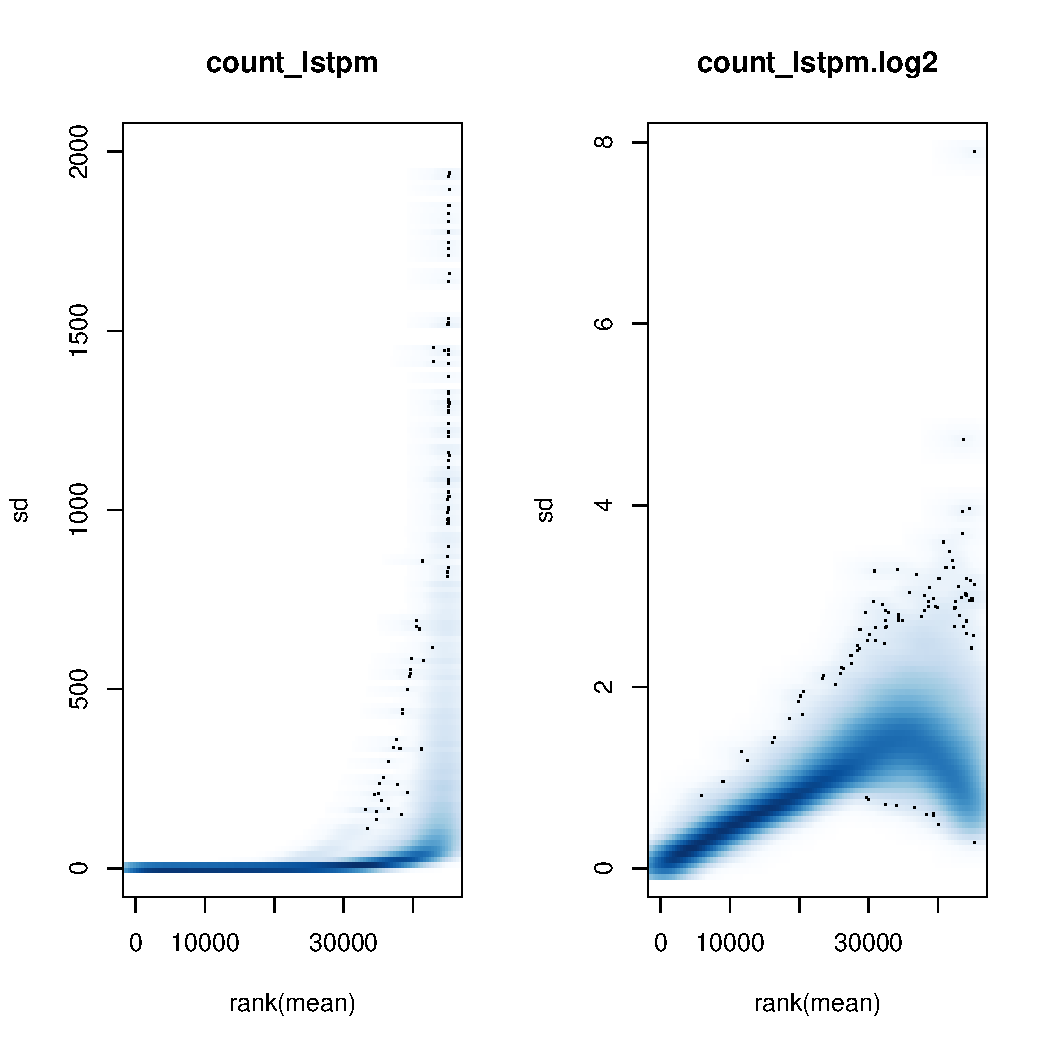
\includegraphics[width=1\linewidth]{/Users/angeloduo/Desktop/masterarbeit/scRNAseq_clustering_comparison/results/QC_data/meanvarplots_kumar2015.pdf}
  \caption{Kumar dataset}
  \label{fig:transsim}
\end{subfigure}%
\begin{subfigure}{.5\textwidth}
  \centering
  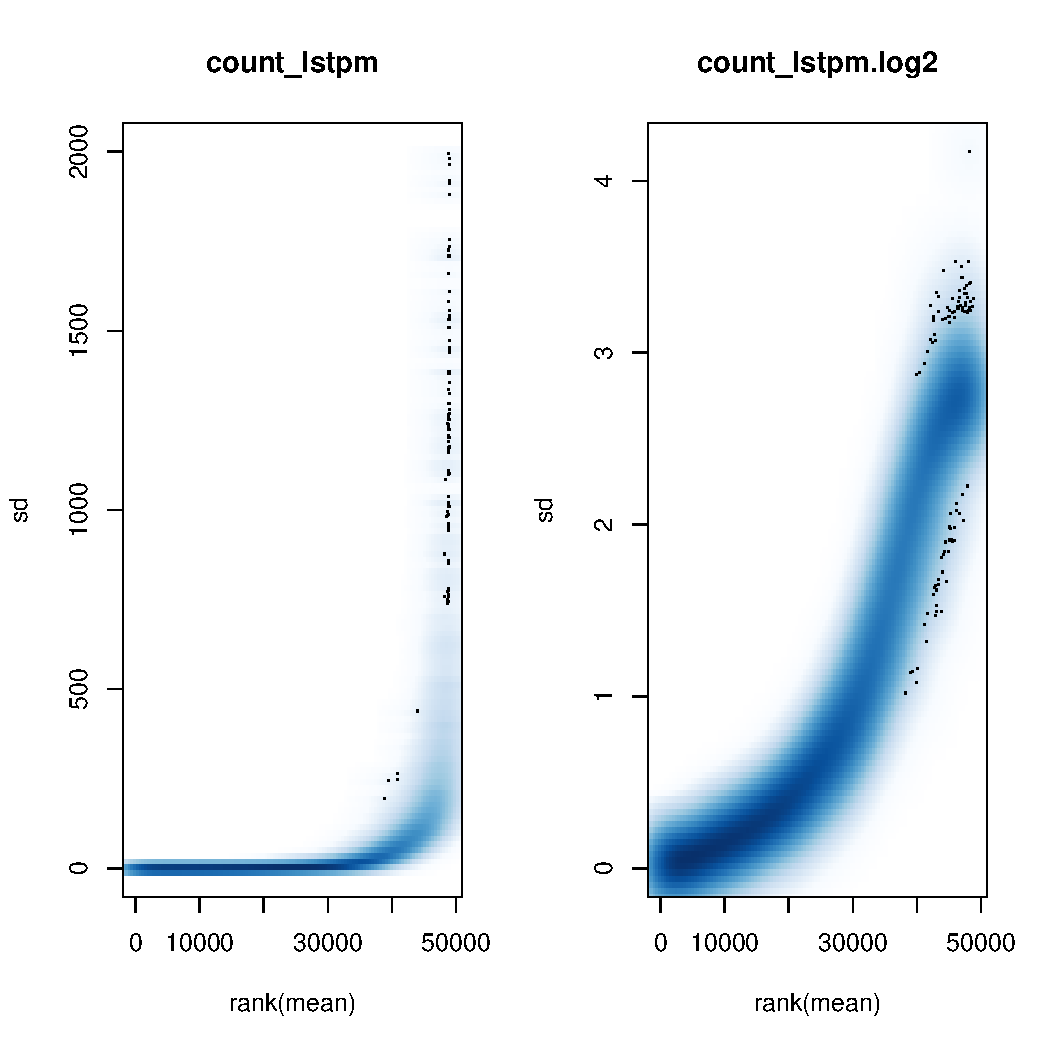
\includegraphics[width=1\linewidth]{/Users/angeloduo/Desktop/masterarbeit/scRNAseq_clustering_comparison/results/QC_data/meanvarplots_koh2016.pdf}
  \caption{Koh dataset}
  \label{fig:transkoh}
\end{subfigure}
\begin{subfigure}{.5\textwidth}
  \centering
  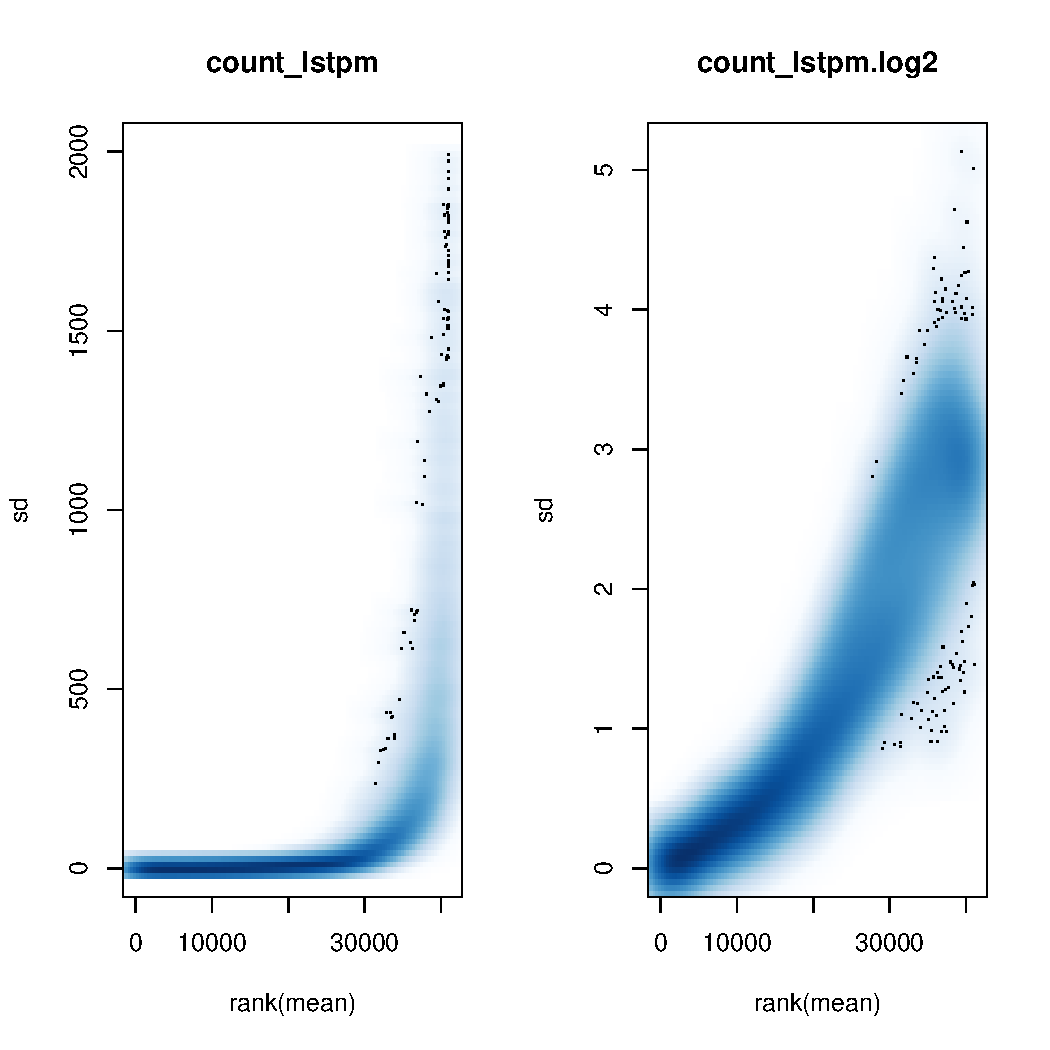
\includegraphics[width=1\linewidth]{/Users/angeloduo/Desktop/masterarbeit/scRNAseq_clustering_comparison/results/QC_data/meanvarplots_trapnell2014.pdf}
  \caption{Trapnell dataset}
  \label{fig:transtrapnell}
\end{subfigure}%
\begin{subfigure}{.5\textwidth}
  \centering
  \includegraphics[width=1\linewidth]{/Users/angeloduo/Desktop/masterarbeit/scRNAseq_clustering_comparison/results/QC_data/meanvarplots_zhengmix2016.pdf}
  \caption{Zheng dataset}
  \label{fig:transzheng}
\end{subfigure}
\caption{Shown is the genewise standart deviation versus the mean for the datasets Kumar (a), Koh(b), Trapnell(c) and Zheng(d). PLotted are the untransformed and the log, arcus sinus and VST-transformed data.  }
\label{fig:trans}
\end{figure}

\newpage
\subsection{Data transformation and normalisation}
\paragraph{Data transformation}
RNA-seq data may suffer from heteroscedasticity and skewness \citep{zwiener2014transforming}. Genes with higher mean have on average a higher variance across cells leading to unequal variances between different genes. 
To handle this property different transformation were considered. Namely, a binary logarithmic transformation with a pseudo-count of one, arcus sinus transformations and a variance-stabilising transformation (VST) from the DESeq package \citep{huber2002variance}. Log transformations will have an impact on extreme values. However, they will not address the problem of heteroscedasticity. Arcus sinus transformation should deal with extreme values and equalise the variances. After transformation, the mean and the variances should be independent. VST addresses the problem of extreme values and unequal variances across genes. After such transformation, the mean and the variances of the genes should be independent. For the study, a binary logarithmic transformation plus a pseudo-count of one is used.  The mean-SD dependence for different transformations is shown in Figure \ref{fig:trans}.

\newpage
\paragraph{Filtering and normalisation}
The quality control of the data sets follows \citet{lun2016step}. In the first step, genes that are not expressed in any cell (systematic--zeros) are removed in order to reduce the size of the expression matrix. To find potential outliers, PCA can be used on the phenotype characteristic of each cell can be used (Figure \ref{fig:qckumar}, \ref{fig:qctrapnell}, \ref{fig:qckoh}, \ref{fig:qczheng}; a). Cells were filtered based on the library size and the total number of genes.
Cells with log10 library sizes that are more than three median absolute deviations (MADs) below the median log-library size were filtered out (Figure \ref{fig:histkumar}, \ref{fig:histtrap}, \ref{fig:histkoh} and \ref{fig:histsim}). The same filter was used with respect to the total number of genes per cell. 
For the Kumar and the Zheng dataset, ERCCs and MT counts were available. Cells with large proportions of ERCC or mitochondrial RNA are seen as low-quality cells. In the Kumar dataset, cells with an ERCC proportion above three MADs are as well removed. The same filter was used for mitochondrial RNA in the Zheng data.

The metadata for the Trapnell dataset contained information about the cell quality. In this dataset, cells that were marked as debris and any single libraries consisting of more than one cell were filtered out. After filtering, 531 cells in the Koh dataset, 246 in the Kumar dataset and 222 in the Trapnell dataset were retained. The filtering was less strict in the Koh dataset compared to the original analysis where they retained 498 cells. 

Low-abundance genes influence the mean-variance trend. Here low-abundance genes are filtered by their average counts (see Figures \ref{fig:qckumar}, \ref{fig:qctrapnell}, \ref{fig:qckoh} and \ref{fig:qczheng}; d ). For the Kumar, Trapnell, simDataKumar and Zheng data genes with average counts less than one are removed. The Zheng data set had a shallower sequencing depth. A different filter is used, and features which are not expressed in at least two cells are excluded.
To find batch effects a linear model regressing the PC values against the total features was used \citep{lun2016step}. 

Another examination of the technical variation was done using the marginal variances\citep{lun2016step}. For that, a linear model with the expression values per gene as response variables and a chosen explanatory variable is fitted. The correlation coefficient can then be seen as the marginal explained variance for the explanatory variables.


A wide variety of normalisation methods exist based on bulk RNA methods. These methods are usually not designed for dealing with the zero-inflated nature of scRNA-seq data\citet{lun2016pooling}. 
Methods for normalisation of scRNA-seq data are based on spike-ins or RNA counts. Spike-in RNA is added before the library preparation. Any changes in the spike-in coverage are assumed to be due to technical factors. The normalisation is done by scaling the counts to level the spike-in. However, this approach is not feasible as none or only a limited number of spike-in counts were present in the datasets.

Here, normalisation through pooled cells is used, where the problem of excess zero counts is reduced by the pooling of multiple cells \citet{lun2016pooling}. The normalisation procedure can briefly be described as follows: (i) Different pools of cells are defined. (ii) The expression values are summed across the cell pools. (iii) The cell pool is normalised against an average of the summed expression values. (iv) This step is repeated several times to construct a linear system. 
The summed count size is then used to estimate the corrected size factor. The size factors for the pooled cells are then deconvoluted" into cell-based factors. 



\begin{figure}[!h]
\includegraphics[width=4 in]{/Users/angeloduo/Desktop/masterarbeit/scRNAseq_clustering_comparison/results/QC_data/hist_Kumar2014.pdf}
\caption{Histogram of Kumar 2014.}
\label{fig:histkumar}
\end{figure}

\begin{figure}[!h]
\includegraphics[width=5 in]{/Users/angeloduo/Desktop/masterarbeit/scRNAseq_clustering_comparison/results/QC_data/hist_Trapnell2014.pdf}
\caption{Histogram of Trapnell 2014. }
\label{fig:histtrap}
\end{figure}

\begin{figure}[!h]
\includegraphics[width=5 in]{/Users/angeloduo/Desktop/masterarbeit/scRNAseq_clustering_comparison/results/QC_data/hist_Koh2016.pdf}
\caption{Histogram of Koh 2016. }
\label{fig:histkoh}
\end{figure}


\begin{figure}[!h]
\includegraphics[width=5 in]{/Users/angeloduo/Desktop/masterarbeit/scRNAseq_clustering_comparison/results/QC_data/hist_simDataKumar.pdf}
\caption{Histogram of simDataKumar. }
\label{fig:histsim}
\end{figure}



\begin{figure}[!h]
\includegraphics[width=5 in]{/Users/angeloduo/Desktop/masterarbeit/scRNAseq_clustering_comparison/results/QC_data/comparison_panel.png}
\caption{Comparison between the data sets. Based on compare function of Splatter.}
\label{fig:compare}
\end{figure}

\begin{figure}[!h]
\includegraphics[width=5 in]{/Users/angeloduo/Desktop/masterarbeit/scRNAseq_clustering_comparison/results/QC_data/qc_summary_kumar.png}
\caption{QC summary of Kumar 2015. }
\label{fig:qckumar}
\end{figure}

\begin{figure}[!h]
\includegraphics[width=5 in]{/Users/angeloduo/Desktop/masterarbeit/scRNAseq_clustering_comparison/results/QC_data/qc_summary_trapnell.png}
\caption{QC summary of Trapnell 2014. }
\label{fig:qctrapnell}
\end{figure}

\begin{figure}[!h]
\includegraphics[width=5 in]{/Users/angeloduo/Desktop/masterarbeit/scRNAseq_clustering_comparison/results/QC_data/qc_summary_koh.png}
\caption{QC summary of Koh 2016. }
\label{fig:qckoh}
\end{figure}

\begin{figure}[!h]
\includegraphics[width=5 in]{/Users/angeloduo/Desktop/masterarbeit/scRNAseq_clustering_comparison/results/QC_data/qc_summary_zheng2016.png}
\caption{QC summary of Zheng 2016. }
\label{fig:qczheng}
\end{figure}

\begin{figure}[!h]
\includegraphics[width=5 in]{/Users/angeloduo/Desktop/masterarbeit/scRNAseq_clustering_comparison/results/QC_data/qc_summary_simDataKumar.png}
\caption{QC summary of simDataKumar. }
\label{fig:simDataKumar}
\end{figure}

\begin{figure}[!h]
\includegraphics[width=5 in]{/Users/angeloduo/Desktop/masterarbeit/scRNAseq_clustering_comparison/results/QC_data/qc_summary_simDataKumar2.png}
\caption{QC summary of simDataKumar2. }
\label{fig:simDataKumar}
\end{figure}


\subsection{Optimal number of clusters}
Methods to determine the optimal number of clusters are subjective methods as elbow or silhouette plots. In the Elbow plots, the within-cluster sum of square is plotted against a range of clusters. The silhouette plot is a standardized measure of distances between each point inside and outside of the respective cluster. Less subjective is the gap statistic. Here the log within sum of squares is compared to its expectation. The null distribution is expected to be uniformly distributed, it is not clear if this is correct for high dimensional data \citep{tibshirani2001estimating}. Other possible methods are the calinsky criterion, hierarchical clustering....
Here the optimal number of clusters is determined by Elbow plots, clustering is based on kmeans clustering and the within-cluster sum of square thereof.
The elbow plots suggest three clusters for the Kumar dataset, 2 - 5 in the Trapnell data, 3 in in the Zhengmix data (see Figure \ref{fig:transkumar} ). The optimal number of clusters is unclear for the Koh data set. 
Minimization of within sum of squares was also done in the tSNE latent space with 30 dimensions. Here the optimal number of clusters are 3,3, 4 and 6 to 8  in the Kumar, Trapnell, Zheng and the Koh data sets, respectively.

\begin{figure}[!h]
\includegraphics[width=5 in]{/Users/angeloduo/Desktop/masterarbeit/scRNAseq_clustering_comparison/results/plots/optimalk_wss_tsnekmeans.pdf}
\caption{Optimal number of clusters by minimizing within sum of squares based on the latent space of tSNE (30 dimensions) }
\label{fig:wsstsne}
\end{figure}

\begin{figure}[!h]
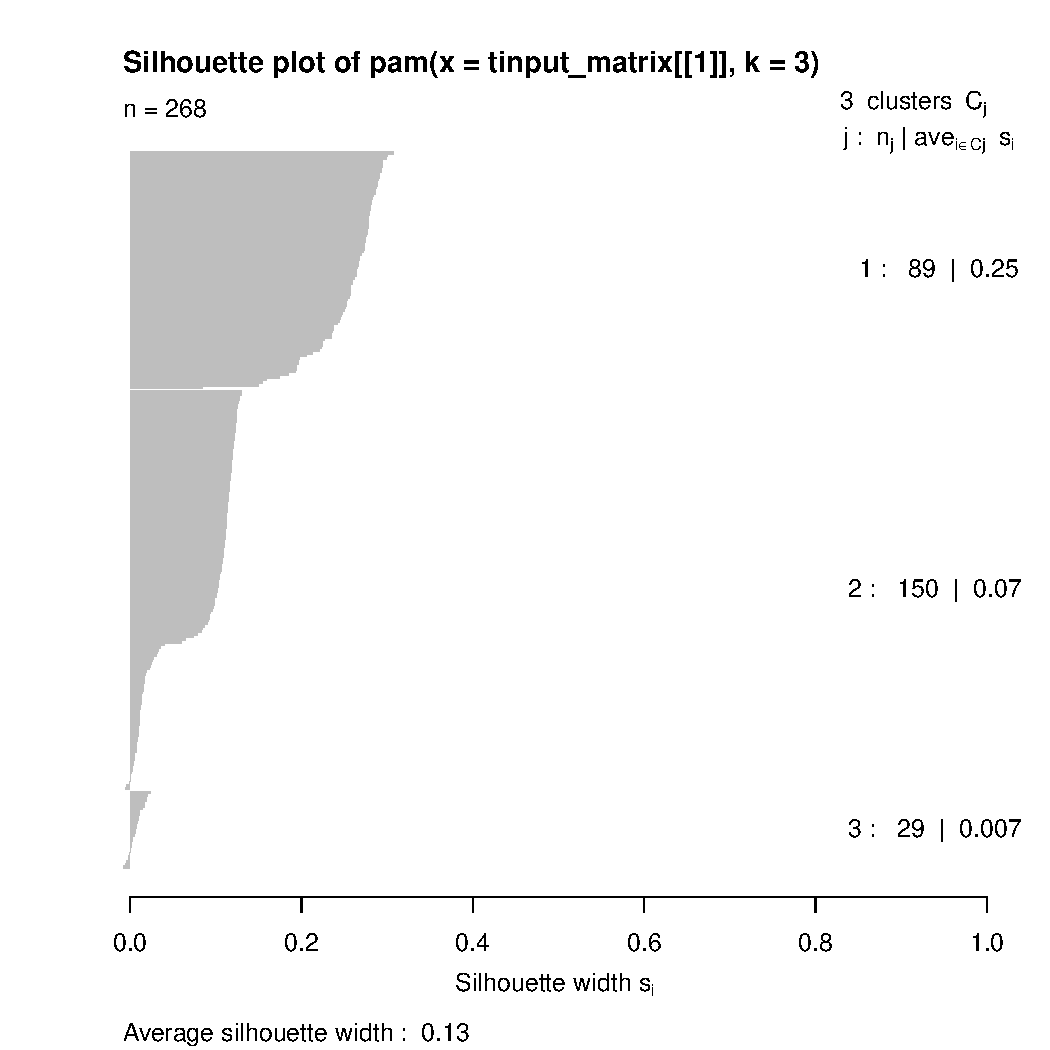
\includegraphics[width=5 in]{/Users/angeloduo/Desktop/masterarbeit/scRNAseq_clustering_comparison/results/plots/optimalk_wss.pdf}
\caption{Optimal number of clusters by within sum of squares based on the full dimensions }
\label{fig:wssorg}
\end{figure}

\newpage
\section{Method}

\begin{center}
\begin{table}[!h]
\footnotesize
\begin{tabular}{ | p{ 2 cm} |  p{ 5 cm}  | p{ 2 cm} | p{ 2 cm} | p{ 0.5 cm} | p{ 0.6 cm} | p{ 0.6 cm} |}
    \hline
    Method & Description & dimension reduction & clustering & zero inflation & normalization & unsupervised \\ \hline
    \hline
     tSNEkmeans & tSNE dimension reduction and kmeans clustering & tSNE & kmeans & no & no & no \\ \hline
    pcaReduce &PCA dimension reduction and kmeans clustering through an iterative process. Step wise merging of cluster by joint probabilities and reducing the number of dimension by PC with lowest variance & PCA & kmeans, hierarchical clustering & no & no &  \\ \hline
     SC3 & PCA  dimension reduction or Laplacian graph. Kmeans clustering on different dimensions. Hierarchical clustering on consensus matrix obtained by kmeans. & PCA & repeated kmeans, hierarchical clustering on similarity matrix of kmeans results & no & no & yes \\ \hline
    SNN-cliq & Shared nearest neighbor  graph based on similarities. Clustering through forming of cliques and subsequent merging. & graph based & merging of cliques & no & no &  \\ \hline
        dbscan & Density based clustering & none &density based clustering & no & no & yes \\ \hline
     SIMLR &  & tSNE & kmeans & yes & no & yes \\ \hline
    CIDR & PCA dimension reduction based on zero imputed similarities. Hierarchical clustering on a number of PC determined by variation of scree method. & PCA on imputed distances & hierarchical clustering& yes & no & yes \\ \hline
   Seurat v1.4 & Nearest neighbor graph based on PCA latent space & HVG and PCA & & no & yes & yes \\ \hline


    \end{tabular}
    \end{table}
\end{center}


\subsection{Evaluation of the clustering methods}

The clustering methods were run with the annotaded number of clusters given by the authors or the truth. Additionally, under default mode and with a maximized ARI. 
The clustering methods were run under the default mode, with cell- and gene-wise filtered data sets and using smoothed data. Additionally, the methods were run under a range of number of clusters.
The run parameters in the default mode were given either by the default setting of the packages or by examples in the different package vignettes. If the method was able to detect the number of subpopulations, the auto detection function was used to infer the number of cluster. For some methods(which) the number of clusters had to be provided. Then, the number of cluster given by the cell annotation provided by the authors were used. 
For the evaluation with filtered data sets filtering steps were excluded. As in the previous evaluation the inputs were counts, log transformed counts and normalized counts. 
Evaluation with non filtered data sets was done as described before, except that the filtering steps are now included in the methods.

Depending on the required inputs counts , log transformed counts  or normalized counts  from the  filtered data sets were used. Any filtering steps done by the methods were excluded in this analysis.

An overview of the different method settings is given by table ...
In a further analysis the clustering methods were tested for different values for the number of clusters $k$. Seurat and dbscan do not allow the setting of the number of cluster. Hence, the number of KNN in Seurat and the size of the neighborhood $\epsilon$ in dbscan was selected.


\subsection{Parameter settings}
For most of the methods the number of cluster is the most important parameter. Other important settings were the kNN, the number of latent space dimensions used for the clustering algorithms or the settings of the filtering and normalization steps.
Here different parameter settings were used to find the optimal settings for each method. First, the methods were run under default mode. Many users will likely run the methods without any fine tuning of the parameters and it was seen important to provide results under this setting. Note that only the methods PCAreduce, SC3, Linnorm, RACEID, TSCAN are completely unsupervised and no parameters have to be provided. For SEURAT and dbscan the number PCs or the number off the kNN have to be defined. CIDR,  RtSNEkmeans, SIMLR need the specification of the number of clusters $k$. For these three methods the parameters setting is equal to the settings described in the next section.
Although its possible to run the methods unsupervised, for many of the methods a fine tuning of the parameters is highly recommended.
Next, methods were run with a the set ground truth of numbers of sub populations. For many of the methods $k$ is a input parameter. However, the methods dbscan and SEURAT allow the setting of $k$ only indirect trough kNN or a resolution parameter. 
To evaluate the methods for the best possible partitions of cells , given the ground truth and evaluated by the use of the ARI score the methods were run under a range of parameters. Whenever possible, the range was chosen such that a clear maximum for the ARI score could be found. A full listing of the parameter settings for each method and run mode is provided in table \ldots .
Next, a brief overview for the chosen parameter setting and the rationale behind it is given.
\paragraph{RtSNEkmeans}
To reduce run time the Barnes-Hut tSNE implementation is used. Perplexity was set to 30 for all data sets. We note that the value of the perplexity can give different tSNE representations, however here the default setting was chosen. tSNE is performed on the first 30 dimensions in the in the PCA latent space .

\paragraph{pcaReduce}
For PCAreduce the range of clusters cannot be specified, instead the number of dimension $q$ in the PCA latent space are to be specified. The results are $q-1$ different clustering solutions, with $k-2$ clusters. For all data sets 30 dimensions were chosen and evaluation was based on the respective number of clusters in the subsequent analysis. The method is based on kmeans clustering and has to be run several times for stable results. Here 50 samples were chosen. Merging of clusters was done by the default sampling proportional to the joint probabilities. 
\paragraph{SC3}
A gene filtering step is implemented in the method.  Filtering steps were included when run with the unfiltered data sets, otherwise the filtering step is excluded. Based on the dropout distribution genes below and above the 10th and 90th percentile  are filtered out before clustering. This seems reasonable for the Kumar, simDataKumar and Koh data sets. However, for the Koh and Zhengmix data set the upper threshold is set to the 99th percentile.
SC3 can run under semi- or unsupervised mode. For the default mode a range of cluster is given, and the number of sub populations is automatically inferred by the method. Otherwise the number of annotated number of sub population is provided. 
\paragraph{SNNCliq}
The connectivity of the quasi-cliques was set to the default value 0.7. Like wise the merging threshold parameter was set to the default of 0.5. The method was run with normalized, filtered data and the number of clusters was set to a range from 3 to 10 in all data sets. SNNclique works on different distance metrics, here the default euclidean distances are used.
\paragraph{SIMLR}
The tuning parameter $k$ was set to the default value of 10 on all runs. The parameter number of clusters $c$ is set accordingly to the run mode.
\paragraph{Seurat}
Implemented in the method are normalization and a gene filtering steps. Filtering criteria are the minimal number of gene expression in the cells and the number of total features per cell. The default setting is zero for both parameters, removing the filtering step. This setting is also chosen when the method is run on the filtered data sets. For the unfiltered data genes which are expressed in less than 5 cells in the Kumar , Trapnell, Koh and simDataKumar were filtered out. For the Zhengmix data the threshold is set to one, according to the filtering used in the QC and normalization steps.
The default log normalization is used, currently the only option. Scale factor for cell-level normalization was set to 10000. As a default no explanatory variables were chosen to be regressed out. The experimental batch would be a natural choice as a covariate, but as the sub populations and the batches are identical for the Kumar and Trapnell data it was chosen not include it. 
The clustering parameters to be defined were a resolution parameter and the number of PCs for the clustering. The resolution parameter was set to the default value of 0.8 . The number of PC was determined by the methods recommended by the authors. Using scree plots and a jackknife permutation test (more exact) to determine the number of principal components. 9, 12, 10 and 15 principal components were used for the Kumar, Trapnell, Zheng and Koh dataset, respectively.
10 percent of cells were used for the number of neighbors in the k-nearest neighbor algorithm. A range of kNN fractions was used to find the the optimal value for the kNN parameter.  A range from 0.5 \% to 40 \% of the total number of cells is used to infer the optimal number for the kNN parameter.
\paragraph{dbscan}
To choose appropriate parameters for the size of neighborhood epsilon and the minimum number of points in neighborhood the k-nearest neighbor distance is used. As a initial number of neighbors 10 percent of cells is used. then for each point the k-NN distance is computed and plot by increasing order. The chosen values for the distances are 280, 410, 35 and 380 for the Kumar, Trapnell, Zheng and Koh data sets, respectively.
The default value for the minimum number of points is 5.
For each of the dataset a range of epsilon around the theoretical optimum was chosen to optimize the clustering results.
\paragraph{CIDR}
CIDR uses three parameter settings; the number of clusters, the number of PCs (nPCs) and the method for hierarchical clustering. By default Ward distances are used in the hierarchical clustering. CIDR is able to infer the number of from 2 to $n$ clusters. By default $n$ is set to $nPC*2+2$. When not run in the default mode we choose the nPC according to a variation of the scree-plot and set the number of cluster accordingly to the respective data set. The number of used PCs for the data sets Kumar, Trapnell, Koh , Zhengmix and simDataKumar are  5, 10, 8, 8 and 3 , respectively.
\paragraph{TSCAN}
The expression matrix is by the default log2 + 1 transformed. In all settings this transformation is used. 
Next, in a filtering step a gene wise threshold for the minimum expression value and a lower bound for the minimum retained fraction of genes that show expression greater than the threshold. As default the minimum expression is set 1 for the transformed counts,  and the minimum fraction is 0.5. The minimum fraction had is set to 0.1 for Zhengmix due to the low sequencing depth of this dataset. For all run methods PCA is performed by default. By default the method infers clusters from a range of 2 to 9 clusters. If run semi supervised the respective number of clusters is given. By default "ellipsoidal, varying volume, shape, and orientation" is used for the model.
\paragraph{Linnorm}
The filtering thresholds are set to the default in all runs, except the Zhengmix data.  For this data set the minimum non-zero expression is to a proportion of 0.1. In the default unsupervised mode the tSNE clustering is performed with $k$ from 2 to 20. In the other runs the respective $k$ per dataset is supplied.
\subsection{Evaluation metrics}
One evaluation criteria was the Hubert - Arabje Adjusted Rand Index (ARI) for comparing two partitions. The measure is adjusted for chance and 0 if there's no agreement between pairs and 1 if there is full agreement between pairs. The other criteria is the F1 score. It is the weighted average mean between precision and recall. With weights defined by the inverse of the precision and recall. F1 scores can take on values between 0 and 1.The predicted clusters and the "ground truth" were match by the Hungarian algorithm. Some of the clustering methods are unsupervised and the partitions does not need to have the same sizes (non-bipartite). This causes problems with Hungarian algorithm. As a solution the assignment matrix is augmented with dummy columns with the maximum matrix value as its entries.




\begin{kframe}


{\ttfamily\noindent\bfseries\color{errorcolor}{\#\# Error in `align<-.xtable`(`*tmp*`, value = switch(1 + is.null(align), : "{}align"{} must have length equal to 5 ( ncol(x) + 1 )}}\end{kframe}



% latex table generated in R 3.4.2 by xtable 1.8-2 package
% Sun Jan  7 11:20:04 2018
\begin{table}[ht]
\centering
\begin{tabular}{rlllll}
  \hline
 & cellfiltering & genefiltering & normalization & autodetect & expressionvalues \\ 
  \hline
tSNEkmeans & no & no & no & no & normcounts \\ 
  pcaReduce & no & no & no & no & normcounts \\ 
  SC3 & no & (yes) & no & yes & normcounts \\ 
  SNNCliq & no & no & no & no & normcounts \\ 
  dbscan & no & no & no & no & normcounts \\ 
  SIMLR & no & no & (yes) & no & normcounts \\ 
  CIDR & no & no & no & yes & normcounts \\ 
  Seurat & (yes) & yes & yes & no & counts \\ 
  TSCAN & no & yes & yes & no & counts \\ 
  ZINBWaVEkmeans & no & no & yes & no & counts \\ 
  RACEID & yes & yes & yes & yes & counts \\ 
  Linnorm & no & (yes) & yes & no & counts \\ 
   \hline
\end{tabular}
\caption{Overview of filtering and normalization steps by method} 
\end{table}


\clearpage

\section{Results}
\paragraph{Transformation and normalisation}
In  Kumar similar amount of the variance is explained by the total number of genes, the proportion of ERCC and the phenotype. This indicates that the data set is heavily influenced by batch effects. The same holds in the Trapnell data, but on a lower scale. Variance in Koh data is primarily influenced by the phenotype and to a lesser extent by the total number of genes and the top 200 features. 
Zheng is primarily dominated by the biological variation with the other explanatory factors contribution only marginally to the total variances.
(Different methods exist to normalize RNA-seq data like TMM normalization, DEseq normalization and by library size. However, none of these methods are designed to deal with the zero-inflated nature of scRNA-seq data\citet{lun2016pooling}.
Another often used approach for scRAN-seq data is the normalization by spike-inn. This approach is not feasible as no or only a limited number of spike-inn counts were present in the data sets.)
The data still shows heteroscedasticity. There are only subtle differences between the arcus sinus and log transformations in all the datasets. The Compared with the Arcus sinus transformation.
\paragraph{Clustering}
The annotated number of clusters in the  Kumar, Trapnell and Koh data sets are 3, 3 and 10, respectively. 
In this data sets the true cell population is  given by the authors annotation and it was  chosen as the ground truth. For the simulated data set simDataKumar the number of sub populations are set to 4. The Zheng dataset contained 4 merged cell sub populations. 
For comparison the within sum of squares (WSS) on a range of kmeans clustering was computed.  Similar results were obtained, with exception of the Koh data where the elbow plots suggest 8 clusters.   

For the  methods cidr, pcaReduce, tSNE and kmeans, SC3 , TSCAN , linnorm and SIMLR a range of number of clusters were used. For Seurat a range in k-NN and for dbscan different neighborhood sizes were picked. The Adjusted Rand Index (ARI) is used as a evaluation metric, with the ground truth set by the cell annotation or the given ground truth.

In the Kumar dataset most of the methods show a clear maximum ARI score with three clusters. An exception is pcaReduce where either 3 and 4 clusters achieved a high score. SC3 has it’s maximum with 3 clusters, but higher numbers of clusters reach as well relatively high scores (see Figure \ref{fig:arirangeall}; a). (In SNNClique almost half of all the clustering labels are in disagreement with the annotated cell labeling.)
CIDR, pcaReduce, tSNEkmeans show a maximum score with three clusters in the Trapnell dataset. Whereas for SIMLR and SC3 the optimal number of clusters is 4 and 2 , respectively . 
In the Zheng data CIDR, Linnorm, pcaReduce,  simlr, tSNEkmeans and SC3 had a maximum score value with 4 clusters.  SC3 reached  similar high values for 4 to 7 clusters. In the Koh data pcaReduce, RtSNEkmeans, SC3, SIMLR, cidr and tscan have their maximum at 10, 12, 11 , 8 , 8 and 10 , respectively. Note that the the maximum is not so clear. Except for CIDR, which had a low overall score, all methods have high values on 8 to 12 clusters. In the simulated data set only CIDR and SIMLR had its maximum with 4 clusters, whereas Linnorm, pcaReduce, RtSNEkmeans and TSCAN have a maximum at 3. 



\paragraph{Clustering with the annotated number of cluster, under default mode and with unfiltered data sets}
All methods were run with the number of cluster set to the annotation given by the authors or by the set ground truth. For graph based methods were the neighborhood size had to be define 10 percent of the total cells were used as the  neighborhood size. Others parameters like the number of PC's in Seurat etc. were chosen according to recommendations given by the method manual. For this clustering the filtered dataset was used. 
The partitioning of the clusters were then evaluated using the ARI. Figure \ref{fig:arifilt} shows the Linnorm and pcaReduce performed bad in the simple Kumar dataset.   (why…) No high scores were achieved  in the relatively difficult Trapnell data, with SC3  , RtSNE and Linnorm as the best performing methods. Overall, pcaReduce had the lowest and  SC3  the highest ARI scores  in the filtered data sets. When run under the default method the methods performed similarly. An exception is Linnorm which has higher scores in the Koh, Kumar and simulated data set.
Figure \ref{fig:aridiff1} shows the differences in the ARI scores between the filtered and unfiltered data sets. Here Seurat,  SIMLR and TSCAN perform better in the Koh data. Better scores were also achieved in the Trapnell data by SIMLR, RtSNEkmeans Linnorm and CIDR. Surprisingly RtSNEkmeans had lower scores in the simulated data. As well as pcaReduce in the Kumar and Zhengmix and Linnorm in the Koh, Kumar and simulated data. 
SC3, Seurat, SIMLR, SIMLRlargescale, CIDR and TSCAN performed best with the filtered data sets. Linnorm, pcaReduce, raceID in the filtered dataset. RtSNEkmeans performed similarly under default settings and in the unfiltered data sets.


F1 scores for the Kumar dataset are shown in Figure \ref{}. Most methods are able to assign the correct partitions the three sub populations. However, Linnorm only detected two clusters. pcaReduce is able to correctly partition cluster number three but fails in the sub populations two and three. In the Trapnell data cell population 1 had the highest score. For population 2 and 3 the scores were lower for all methods.
Koh had the highest number cluster, here nine cluster were annotated by the authors. The majority of the methods failed to assign cells to sub population 6 (which is that and why).


\clearpage
\begin{figure}[!h]
\includegraphics[width=5 in]{/Users/angeloduo/Desktop/masterarbeit/scRNAseq_clustering_comparison/results/plots/plot_ari_unfiltered.pdf}
\caption{ARI scores with unfiltered data sets. The number of clusters is determined by the authors annotation. }
\label{fig:ariunfilt}
\end{figure}
\begin{figure}[!h]
\includegraphics[width=5 in]{/Users/angeloduo/Desktop/masterarbeit/scRNAseq_clustering_comparison/results/plots/plot_ari_default.pdf}
\caption{ARI scores with default setting. }
\label{fig:aridef}
\end{figure}

\begin{figure}[!h]
\includegraphics[width=5 in]{/Users/angeloduo/Desktop/masterarbeit/scRNAseq_clustering_comparison/results/plots/plot_ari_filtered.pdf}
\caption{ARI scores with filtered data sets.  The number of clusters is determined by the authors annotation. }
\label{fig:arifilt}
\end{figure}



\begin{figure}[!h]
\includegraphics[width=5 in]{/Users/angeloduo/Desktop/masterarbeit/scRNAseq_clustering_comparison/results/plots/plot_ari_optimalk.pdf}
\caption{ARI scores with filtered data sets. A optimal k is chosen such that the ARI score is maximized. }
\label{fig:arifilt}
\end{figure}

\begin{figure}[!h]
\includegraphics[width=5 in]{/Users/angeloduo/Desktop/masterarbeit/scRNAseq_clustering_comparison/results/plots/plot_ari_smooth.pdf}
\caption{ARI scores with smoothed data sets.  }
\label{fig:arifilt}
\end{figure}


\begin{figure}[!h]
\includegraphics[width=5 in]{/Users/angeloduo/Desktop/masterarbeit/scRNAseq_clustering_comparison/results/plots/plot_ari_rank_all.pdf}
\caption{Ranks of ARI scores.  }
\label{fig:arirank}
\end{figure}

\begin{figure}[!h]
\includegraphics[width=5 in]{/Users/angeloduo/Desktop/masterarbeit/scRNAseq_clustering_comparison/results/plots/plot_ari_stars_all.pdf}
\caption{Starplot of ARI scores.  }
\label{fig:arirank}
\end{figure}


\begin{figure}[!h]
\includegraphics[width=5 in]{/Users/angeloduo/Desktop/masterarbeit/scRNAseq_clustering_comparison/results/plots/plot_ari_diff_maxscore_all.pdf}
\caption{Differences between maximum ARI scores.  }
\label{fig:aridiff1}
\end{figure}

\begin{figure}[!h]
\includegraphics[width=5 in]{/Users/angeloduo/Desktop/masterarbeit/scRNAseq_clustering_comparison/results/plots/plot_ari_diff_all.pdf}
\caption{Differences in ARI scores between  data sets.  }
\label{fig:aridiff1}
\end{figure}



\begin{figure}[!h]
\includegraphics[width=5 in]{/Users/angeloduo/Desktop/masterarbeit/scRNAseq_clustering_comparison/results/plots/plot_ari_krange_ncluster_all.pdf}
\caption{ARI scores for range of parameters for the data sets Kumar (a), Trapnell (b), Zhengmix (c), Koh (d) and simDatakKumar (e). Shown are the methods where the number of cluster could be defined. Shown are the methods...}
\label{fig:arirangeall}
\end{figure}


\begin{figure}[!h]
\includegraphics[width=5 in]{/Users/angeloduo/Desktop/masterarbeit/scRNAseq_clustering_comparison/results/plots/plot_f1_filtered_kumar2015.pdf}
\caption{F1 scores for the filtered Kumar dataset }
\label{fig:f1kumar}
\end{figure}

\begin{figure}[!h]
\includegraphics[width=5 in]{/Users/angeloduo/Desktop/masterarbeit/scRNAseq_clustering_comparison/results/plots/plot_f1_filtered_trapnell2014.pdf}
\caption{F1 scores for  the filtered Trapnell dataset }
\label{fig:f1trapnell}
\end{figure}

\begin{figure}[!h]
\includegraphics[width=5 in]{/Users/angeloduo/Desktop/masterarbeit/scRNAseq_clustering_comparison/results/plots/plot_f1_filtered_koh2016.pdf}
\caption{F1 scores for the filtered Koh dataset }
\label{fig:f1koh}
\end{figure}

\begin{figure}[!h]
\includegraphics[width=5 in]{/Users/angeloduo/Desktop/masterarbeit/scRNAseq_clustering_comparison/results/plots/plot_f1_filtered_zhengmix2016.pdf}
\caption{F1 scores for the filtered Zheng mix dataset }
\label{fig:f1zheng}
\end{figure}

\begin{figure}[!h]
\includegraphics[width=5 in]{/Users/angeloduo/Desktop/masterarbeit/scRNAseq_clustering_comparison/results/plots/plot_f1_filtered_simDataKumar.pdf}
\caption{F1 scores for the filtered simDataKumar. }
\label{fig:f1sim}
\end{figure}


\begin{figure}[!h]
\includegraphics[width=5 in]{/Users/angeloduo/Desktop/masterarbeit/scRNAseq_clustering_comparison/results/plots/runtimes.pdf}
\caption{Runtime for the methods on the data sets Kumar etc. }
\label{fig:runtime}
\end{figure}

\begin{figure}[!h]
\includegraphics[width=5 in]{/Users/angeloduo/Desktop/masterarbeit/scRNAseq_clustering_comparison/results/plots/stability_boot.pdf}
\caption{Stability analysis results with (20) bootstrap samples for the Kumar dataset.}
\label{fig:boot}
\end{figure}

\begin{figure}[!h]
\includegraphics[width=5 in]{/Users/angeloduo/Desktop/masterarbeit/scRNAseq_clustering_comparison/results/plots/stability_subsample_boot.pdf}
\caption{Stability analysis results with 20 subsamples (n=100) for the Kumar dataset.}
\label{fig:stab}
\end{figure}

\begin{figure}[!h]
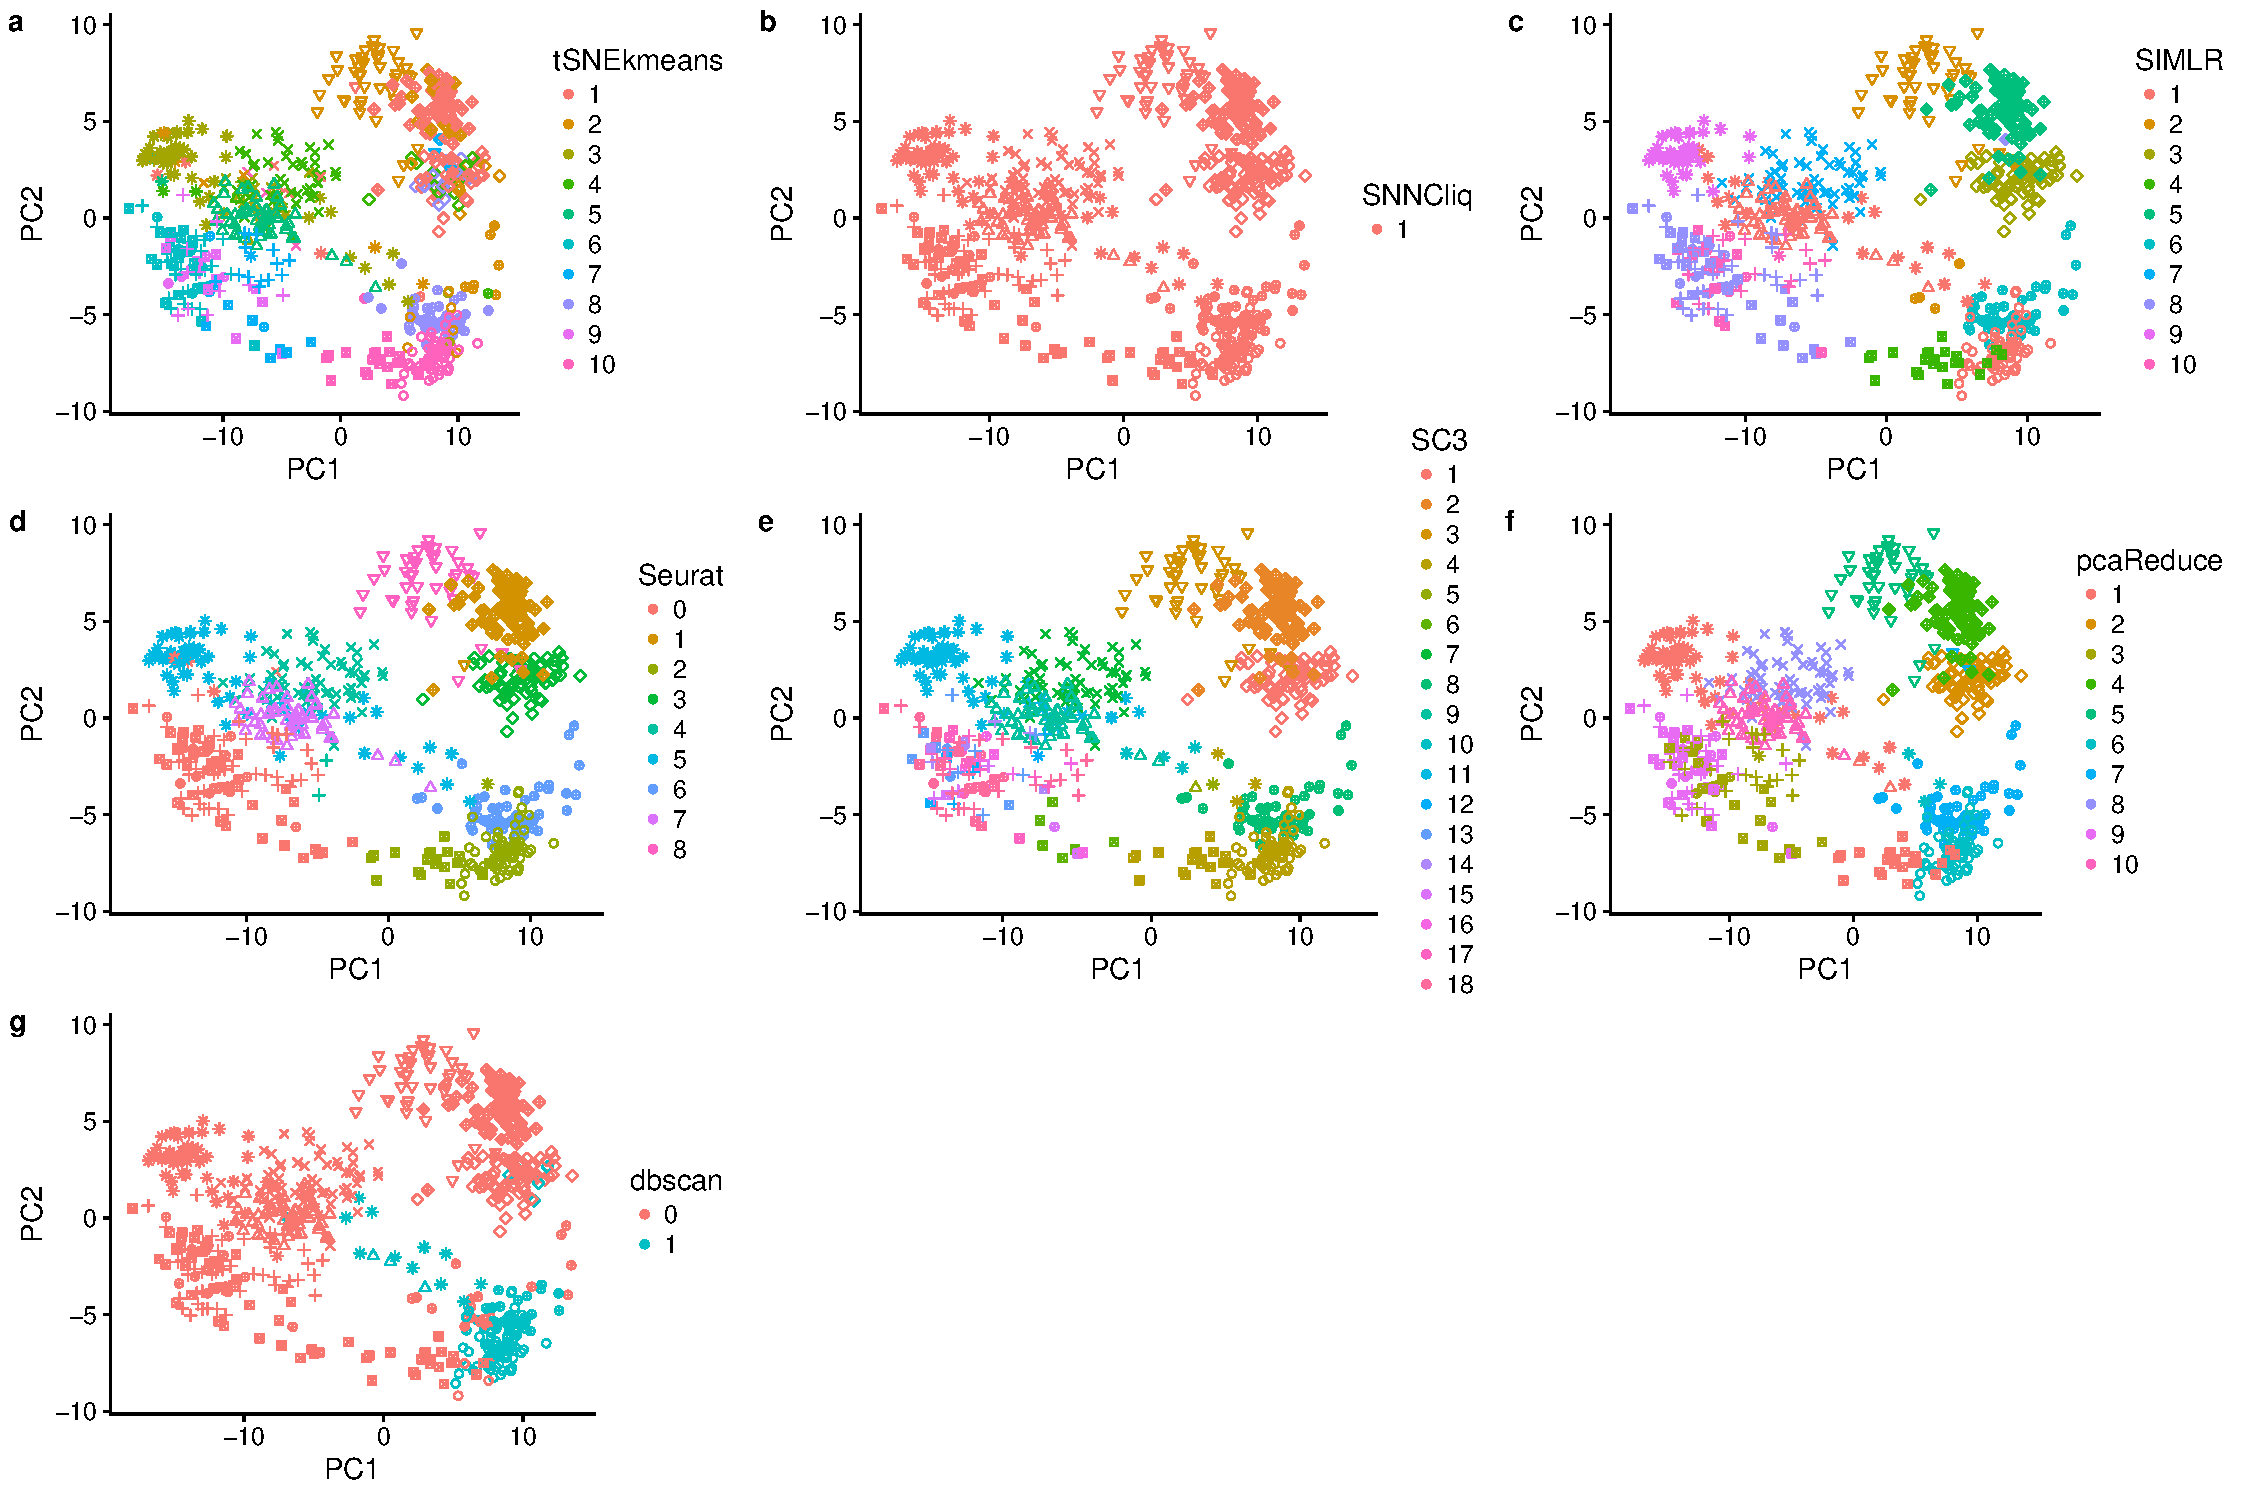
\includegraphics[width=5 in]{/Users/angeloduo/Desktop/masterarbeit/scRNAseq_clustering_comparison/results/plots/plot_cluster_koh2016.pdf}
\caption{Clusters koh2016 on PC representations. }
\label{fig:clusterkoh}
\end{figure}


\begin{figure}[!h]
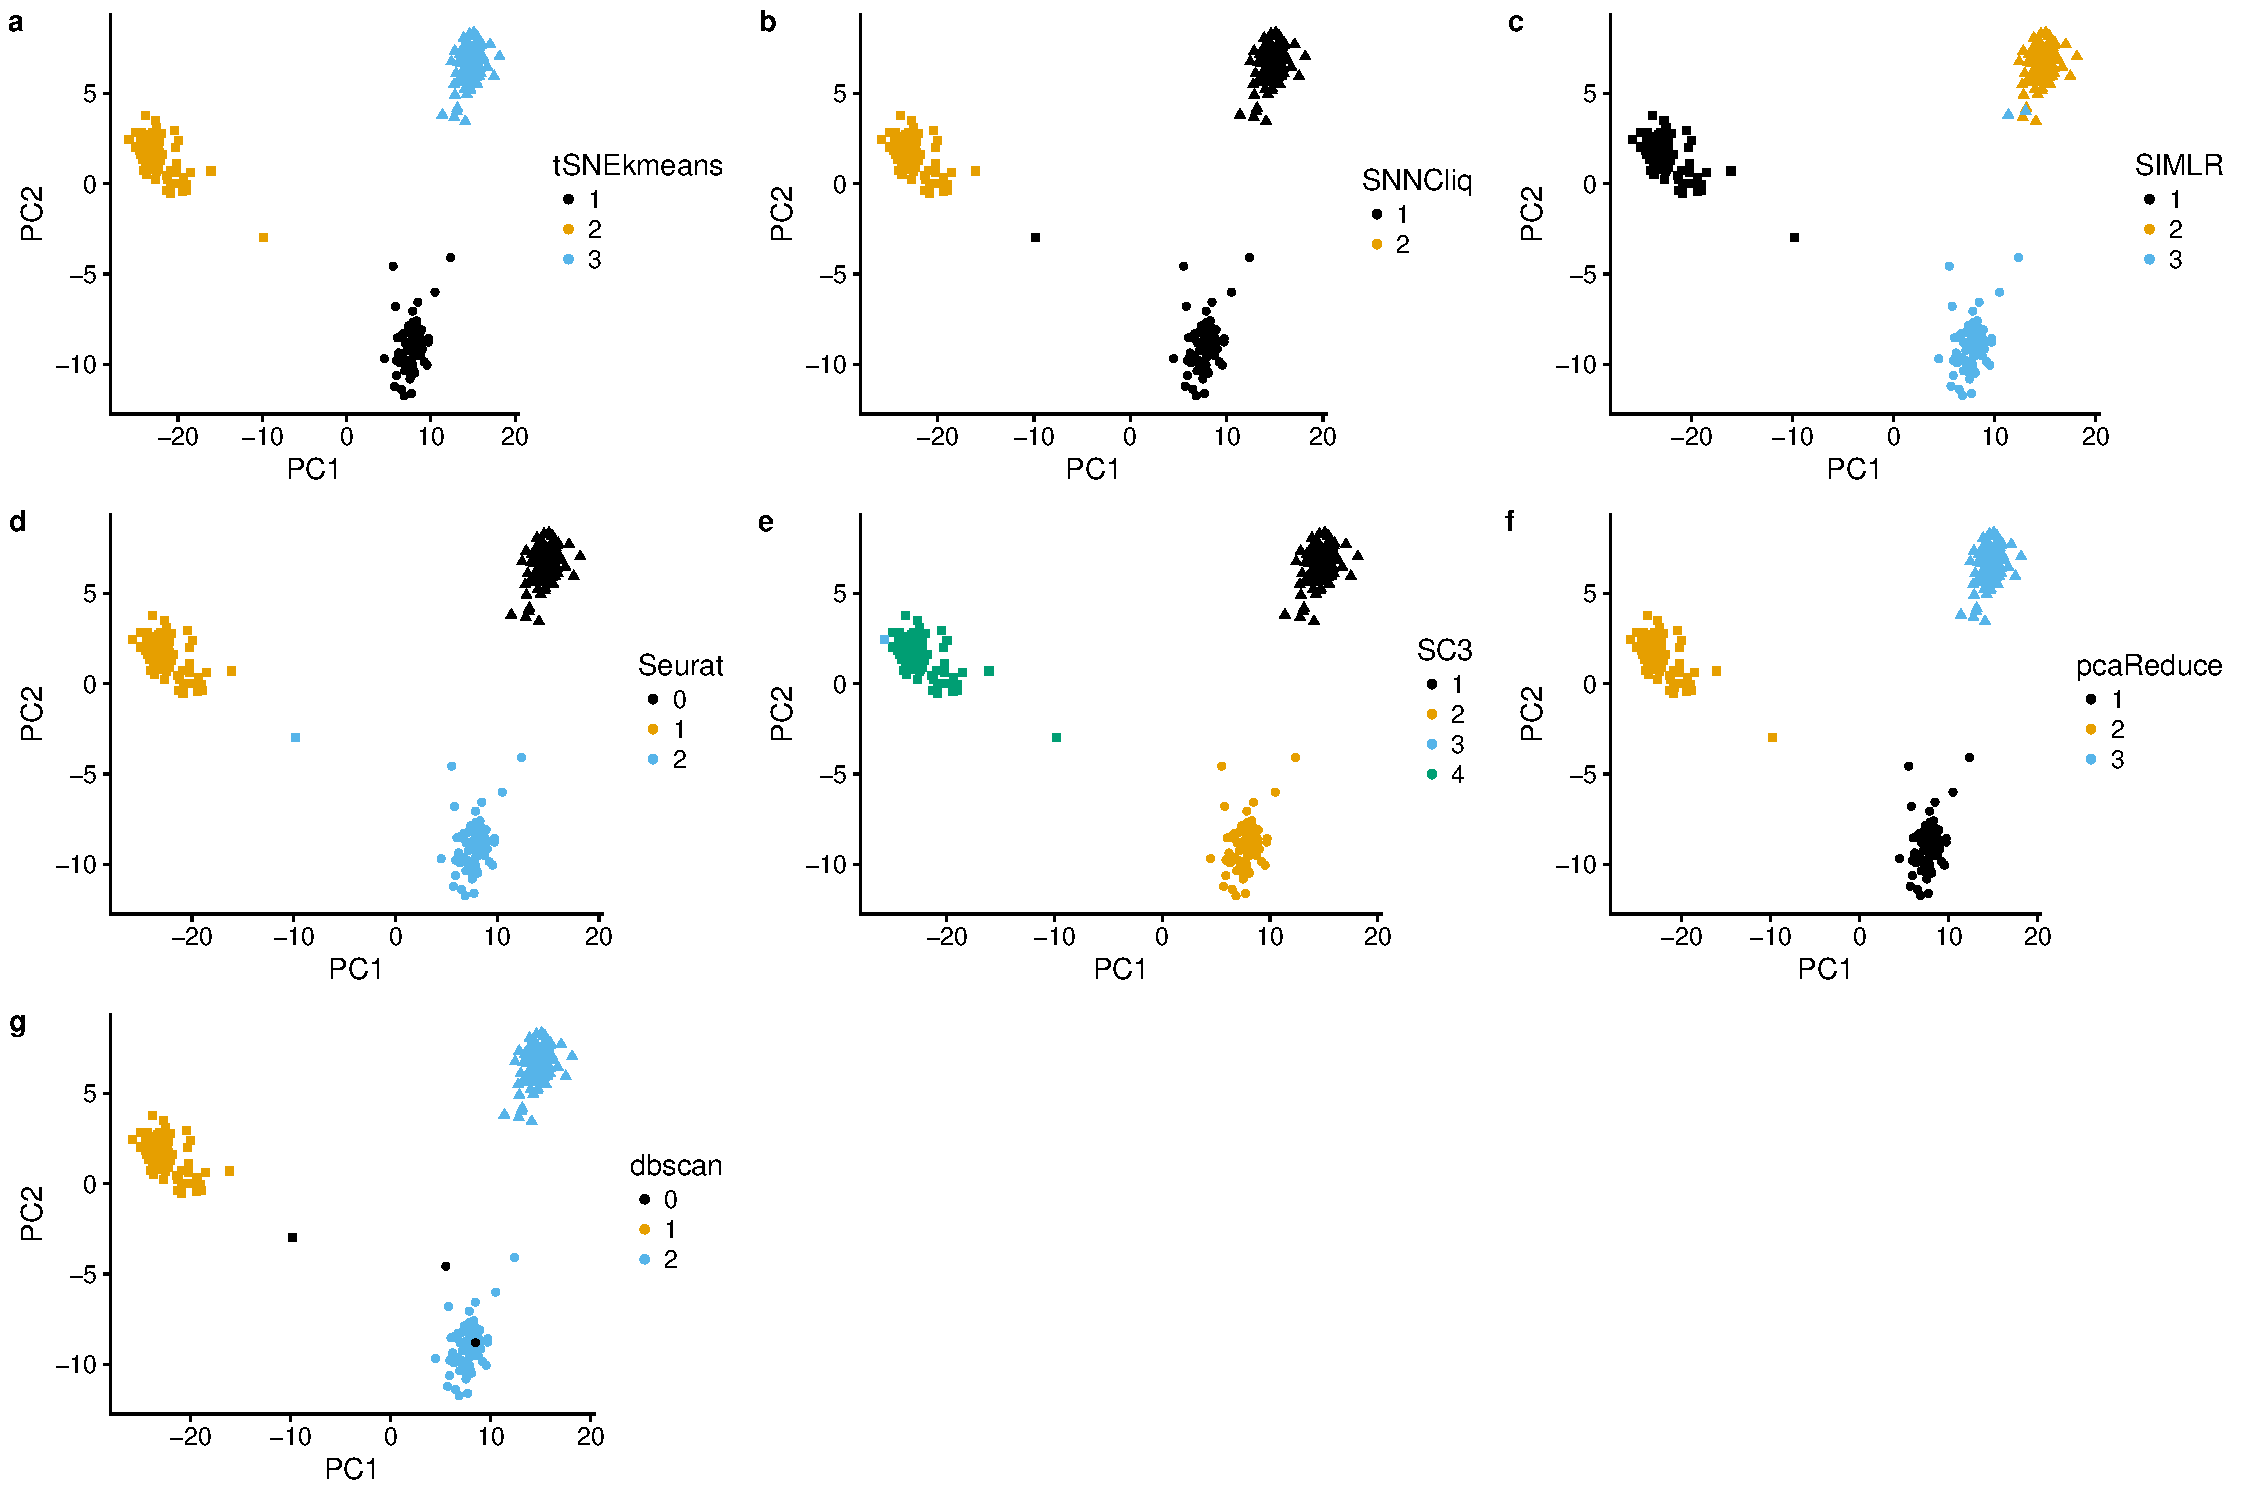
\includegraphics[width=5 in]{/Users/angeloduo/Desktop/masterarbeit/scRNAseq_clustering_comparison/results/plots/plot_cluster_kumar2015.pdf}
\caption{Clusters Kumar 2015 on PC representations. }
\label{fig:clusterkumar}
\end{figure}

\begin{figure}[!h]
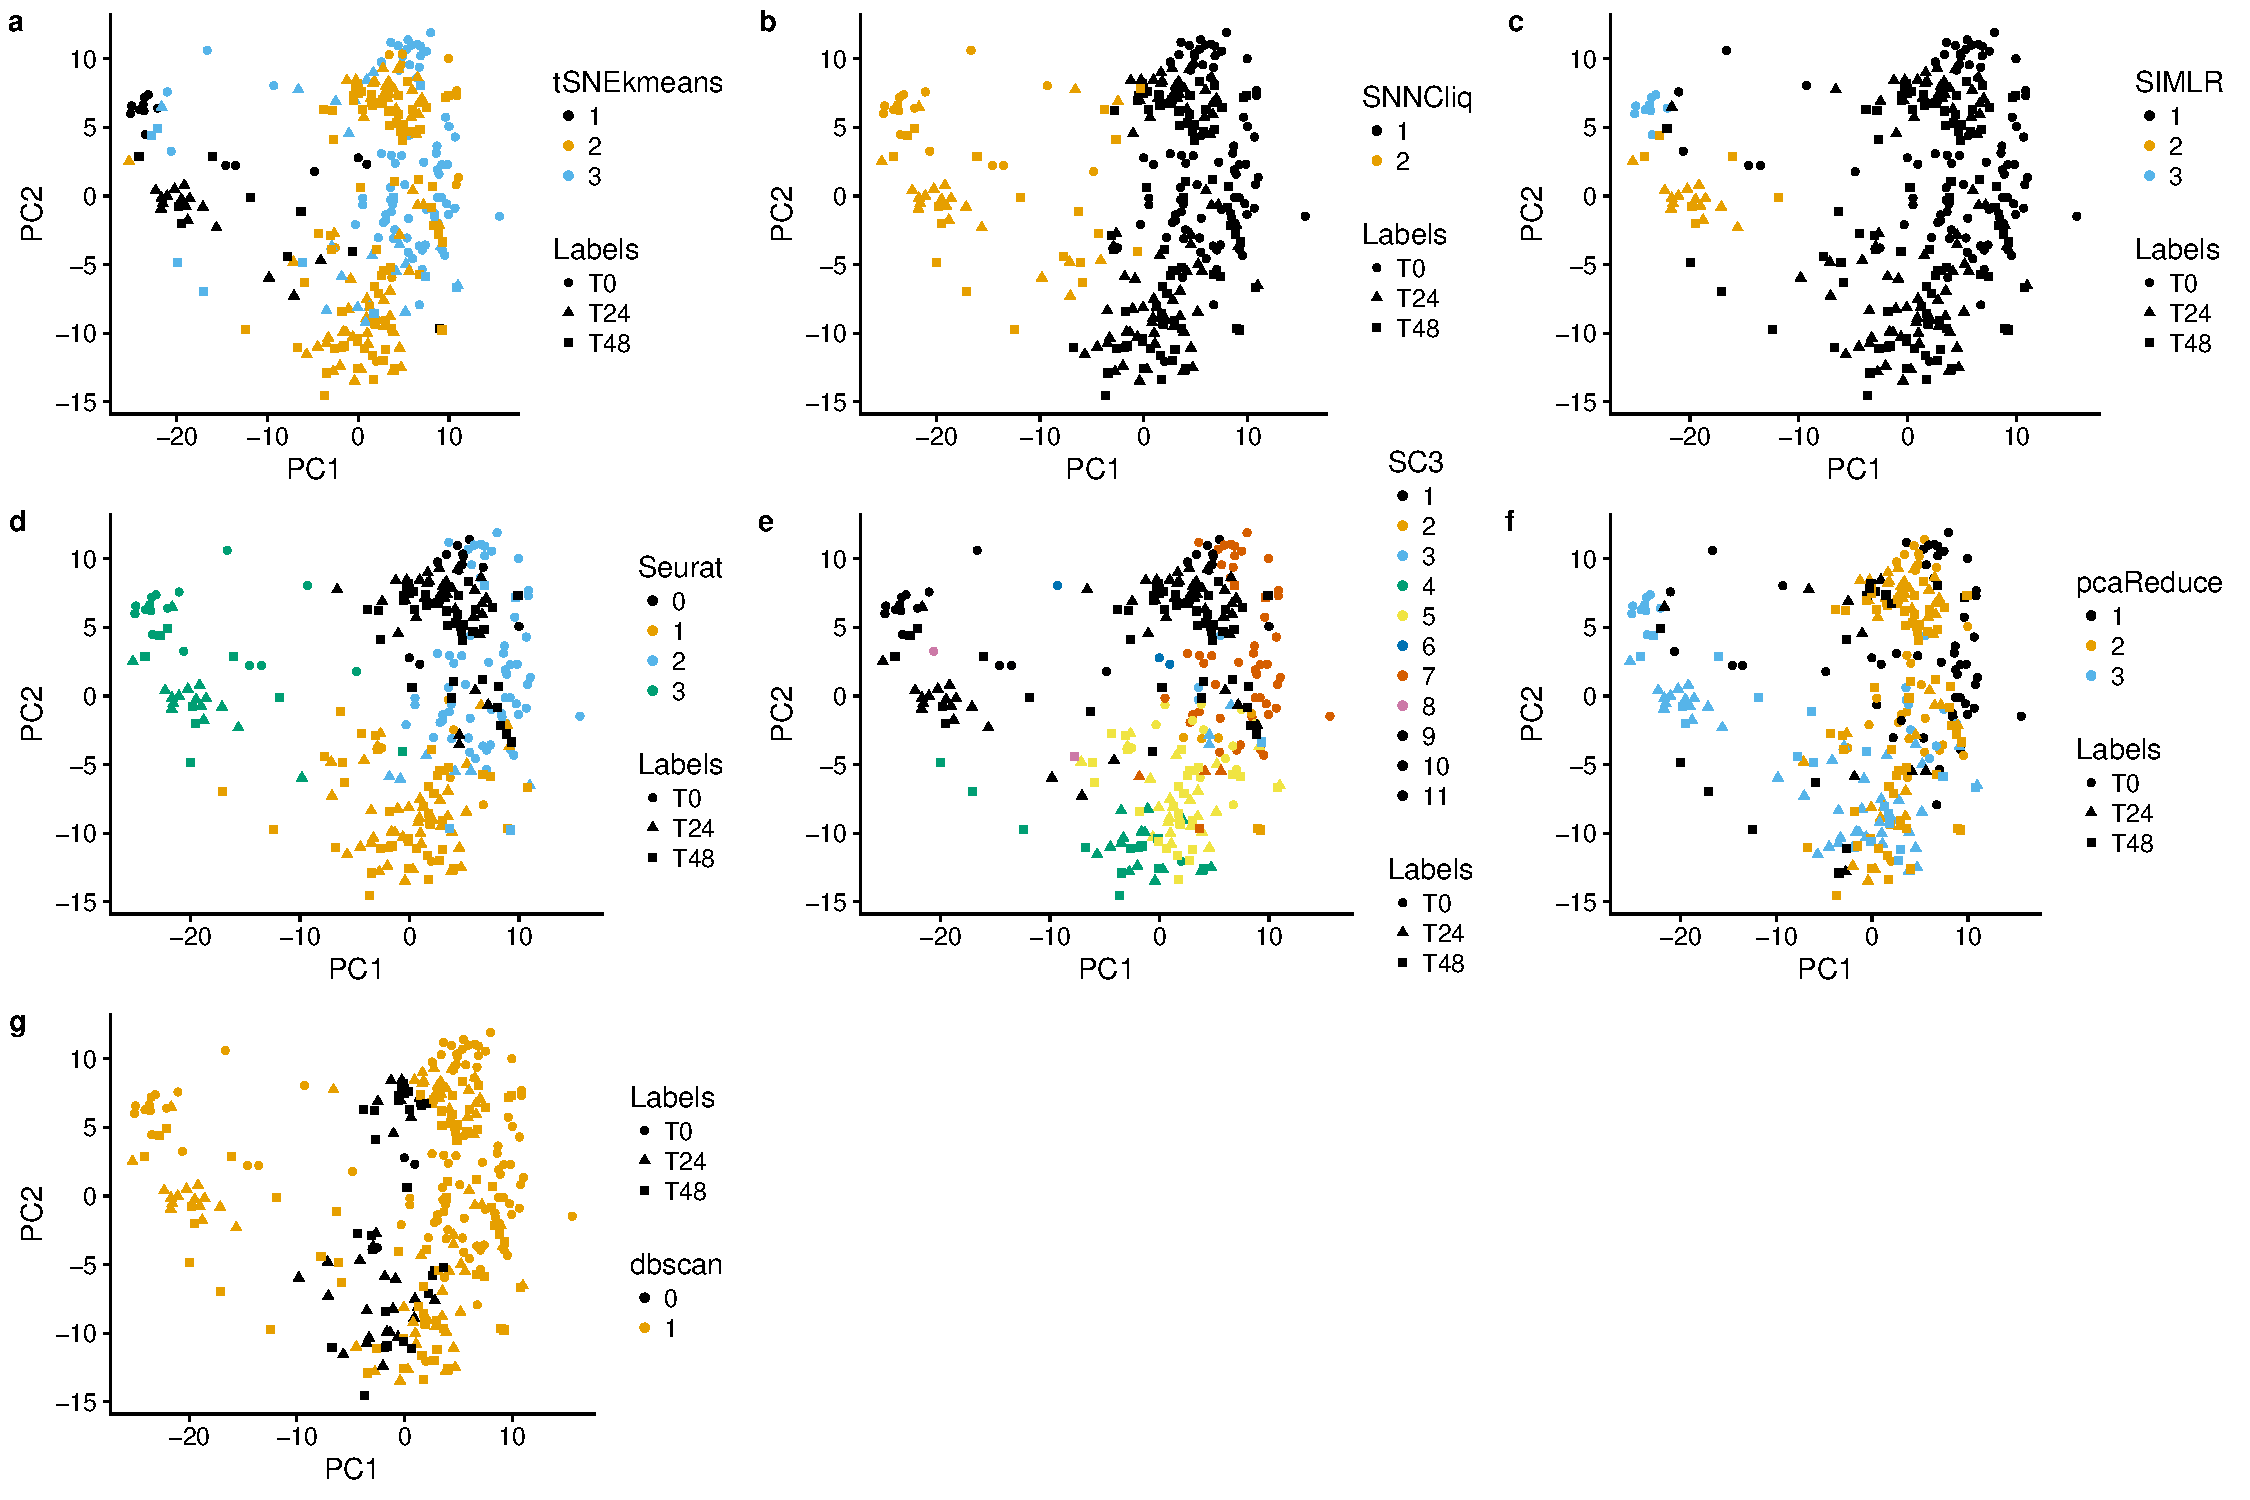
\includegraphics[width=5 in]{/Users/angeloduo/Desktop/masterarbeit/scRNAseq_clustering_comparison/results/plots/plot_cluster_trapnell2014.pdf}
\caption{Clusters Trapnell 2014 on PC representations. }
\label{fig:clustertrapnell}
\end{figure}

\clearpage
\begin{table}[ht]
\centering
\begin{tabular}{rllllll}
  \hline
 & method & parameters & default & annotated k & highest ARI (from k range) & X6 \\ 
  \hline
1 & cidr & n & NULL & NULL &  &  \\ 
  2 & cidr & nCluster & NULL & k &  &  \\ 
  3 & cidr & nPC & 4 & 4 &  &  \\ 
  4 & cidr & cMethod & wardD2 & wardD2 &  &  \\ 
  5 & dbscan & eps & user & user &  &  \\ 
  6 & dbscan & minPts (kNN) & 5 & 0.1 &  &  \\ 
  7 & linnorm & minZeroPortion & 0.75 & 0.75 , (0.25 for Zheng) &  &  \\ 
  8 & linnorm & num\_PC & 3 & 3 &  &  \\ 
  9 & linnorm & num\_Center & 1 to 20 & k &  &  \\ 
  10 & RaceID & min.total & 3000 ( 200 for Zheng) & 3000 ( 200 for Zheng) &  &  \\ 
  11 & RaceID & max.expr & Inf & Inf &  &  \\ 
  12 & RaceID & min.expr & 5 & 5 &  &  \\ 
  13 & RaceID & minnumber & 1 & 1 &  &  \\ 
  14 & RaceID & do.gap & TRUE & FALSE &  &  \\ 
  15 & RaceID & clustrnr & 20 & 0 &  &  \\ 
  16 & RaceID & cln & 0 & k &  &  \\ 
  17 & Rtsnekmeans & k & k & k &  &  \\ 
  18 & Rtsnekmeans & Perplexity & 30 & 30 &  &  \\ 
  19 & Rtsnekmeans & initial\_dims & 50 & 30 &  &  \\ 
  20 & SIMLRlargescale & c & k & k &  &  \\ 
  21 & SIMLRlargescale & k & 10 & 10 &  &  \\ 
  22 & SIMLRlargescale & kk & 100 & 100 &  &  \\ 
  23 & SIMLRlargescale & normalize & FALSE & FALSE &  &  \\ 
  24 & SIMLR & c & k & k &  &  \\ 
  25 & SIMLR & k & 10 & 10 &  &  \\ 
  26 & SIMLR & kk & 100 & 100 &  &  \\ 
  27 & SIMLR & normalize & FALSE & TRUE &  &  \\ 
  28 & SIMLR & no.dim &  &  &  &  \\ 
  29 & tscan & minexpr\_percent & 0.1 to 0.5 & 0.1 to 0.5 &  &  \\ 
  30 & tscan & clusternum & 2 to 20 & k &  &  \\ 
  31 & SC3 & ks & 2 to 10 & elbowplot &  &  \\ 
  32 & SC3 & k\_estimator & TRUE & FALSE &  &  \\ 
  33 & SEURAT & k.param & 30 & 10 percent &  &  \\ 
  34 & SEURAT & dims.use & NULL & screeplot &  &  \\ 
  35 & SEURAT & reduction.type & pca & pca &  &  \\ 
  36 & SEURAT & resolution & 0.8 & 0.8 &  &  \\ 
  37 & pcaReduce & q & 30 & 30 &  &  \\ 
  38 & pcaReduce & nbt & 100 & 100 &  &  \\ 
   \hline
\end{tabular}
\end{table}

% =======================================
% \section{References} \label{sec:ref}
% =======================================
\clearpage

\bibliography{/Users/angeloduo/Desktop/masterarbeit/scRNAseq_clustering_comparison/report/scRNAseq_clustering.bib}


\end{document}
